\documentclass{beamer}\usepackage[]{graphicx}\usepackage[]{xcolor}
% maxwidth is the original width if it is less than linewidth
% otherwise use linewidth (to make sure the graphics do not exceed the margin)
\makeatletter
\def\maxwidth{ %
  \ifdim\Gin@nat@width>\linewidth
    \linewidth
  \else
    \Gin@nat@width
  \fi
}
\makeatother

\definecolor{fgcolor}{rgb}{0.345, 0.345, 0.345}
\newcommand{\hlnum}[1]{\textcolor[rgb]{0.686,0.059,0.569}{#1}}%
\newcommand{\hlstr}[1]{\textcolor[rgb]{0.192,0.494,0.8}{#1}}%
\newcommand{\hlcom}[1]{\textcolor[rgb]{0.678,0.584,0.686}{\textit{#1}}}%
\newcommand{\hlopt}[1]{\textcolor[rgb]{0,0,0}{#1}}%
\newcommand{\hlstd}[1]{\textcolor[rgb]{0.345,0.345,0.345}{#1}}%
\newcommand{\hlkwa}[1]{\textcolor[rgb]{0.161,0.373,0.58}{\textbf{#1}}}%
\newcommand{\hlkwb}[1]{\textcolor[rgb]{0.69,0.353,0.396}{#1}}%
\newcommand{\hlkwc}[1]{\textcolor[rgb]{0.333,0.667,0.333}{#1}}%
\newcommand{\hlkwd}[1]{\textcolor[rgb]{0.737,0.353,0.396}{\textbf{#1}}}%
\let\hlipl\hlkwb

\usepackage{framed}
\makeatletter
\newenvironment{kframe}{%
 \def\at@end@of@kframe{}%
 \ifinner\ifhmode%
  \def\at@end@of@kframe{\end{minipage}}%
  \begin{minipage}{\columnwidth}%
 \fi\fi%
 \def\FrameCommand##1{\hskip\@totalleftmargin \hskip-\fboxsep
 \colorbox{shadecolor}{##1}\hskip-\fboxsep
     % There is no \\@totalrightmargin, so:
     \hskip-\linewidth \hskip-\@totalleftmargin \hskip\columnwidth}%
 \MakeFramed {\advance\hsize-\width
   \@totalleftmargin\z@ \linewidth\hsize
   \@setminipage}}%
 {\par\unskip\endMakeFramed%
 \at@end@of@kframe}
\makeatother

\definecolor{shadecolor}{rgb}{.97, .97, .97}
\definecolor{messagecolor}{rgb}{0, 0, 0}
\definecolor{warningcolor}{rgb}{1, 0, 1}
\definecolor{errorcolor}{rgb}{1, 0, 0}
\newenvironment{knitrout}{}{} % an empty environment to be redefined in TeX

\usepackage{alltt}
\usetheme{warsaw} % {Berkeley} % {Hannover} % {Singapore}
% {CambridgeUS}
\usecolortheme{seahorse}%{rose}
\usefonttheme{professionalfonts} 
\setbeamercovered{dynamic}
% \useinnertheme[shadow]{rounded}


\usepackage{geometry}
\usepackage{inputenc}
\usepackage{algorithm2e}
\usepackage{times}
\usepackage{amsmath, amsfonts, amstext}



%%%%%%%%%%%%%%%%%%%%
\usepackage{bm}
\usepackage{graphicx}
\usepackage{hyperref}
\usepackage{float}
\usepackage{amsmath}
\usepackage{tcolorbox}

\usepackage{amssymb}


\usepackage{tikz}
\usetikzlibrary{shapes.geometric, arrows, matrix}
\usepackage{array}
\usepackage{multicol}
\usepackage{graphicx}
\usepackage{setspace}

\usepackage{caption}



\usepackage{makecell}
\usepackage{color}   %May be necessary if you want to color links
\usepackage{hyperref}
\hypersetup{
    pdfpagemode=FullScreen,
	colorlinks = true, %set true if you want colored links
	linktoc = all,     %set to all if you want both sections and subsections linked
	linkcolor = blue,  %choose some color if you want links to stand out
    citecolor = red
}














%%%%%%%%%%%%



\graphicspath{{./Fig/}}

\date{\small 1402-1403\\[0.5cm]}
\title[R WorkShop]{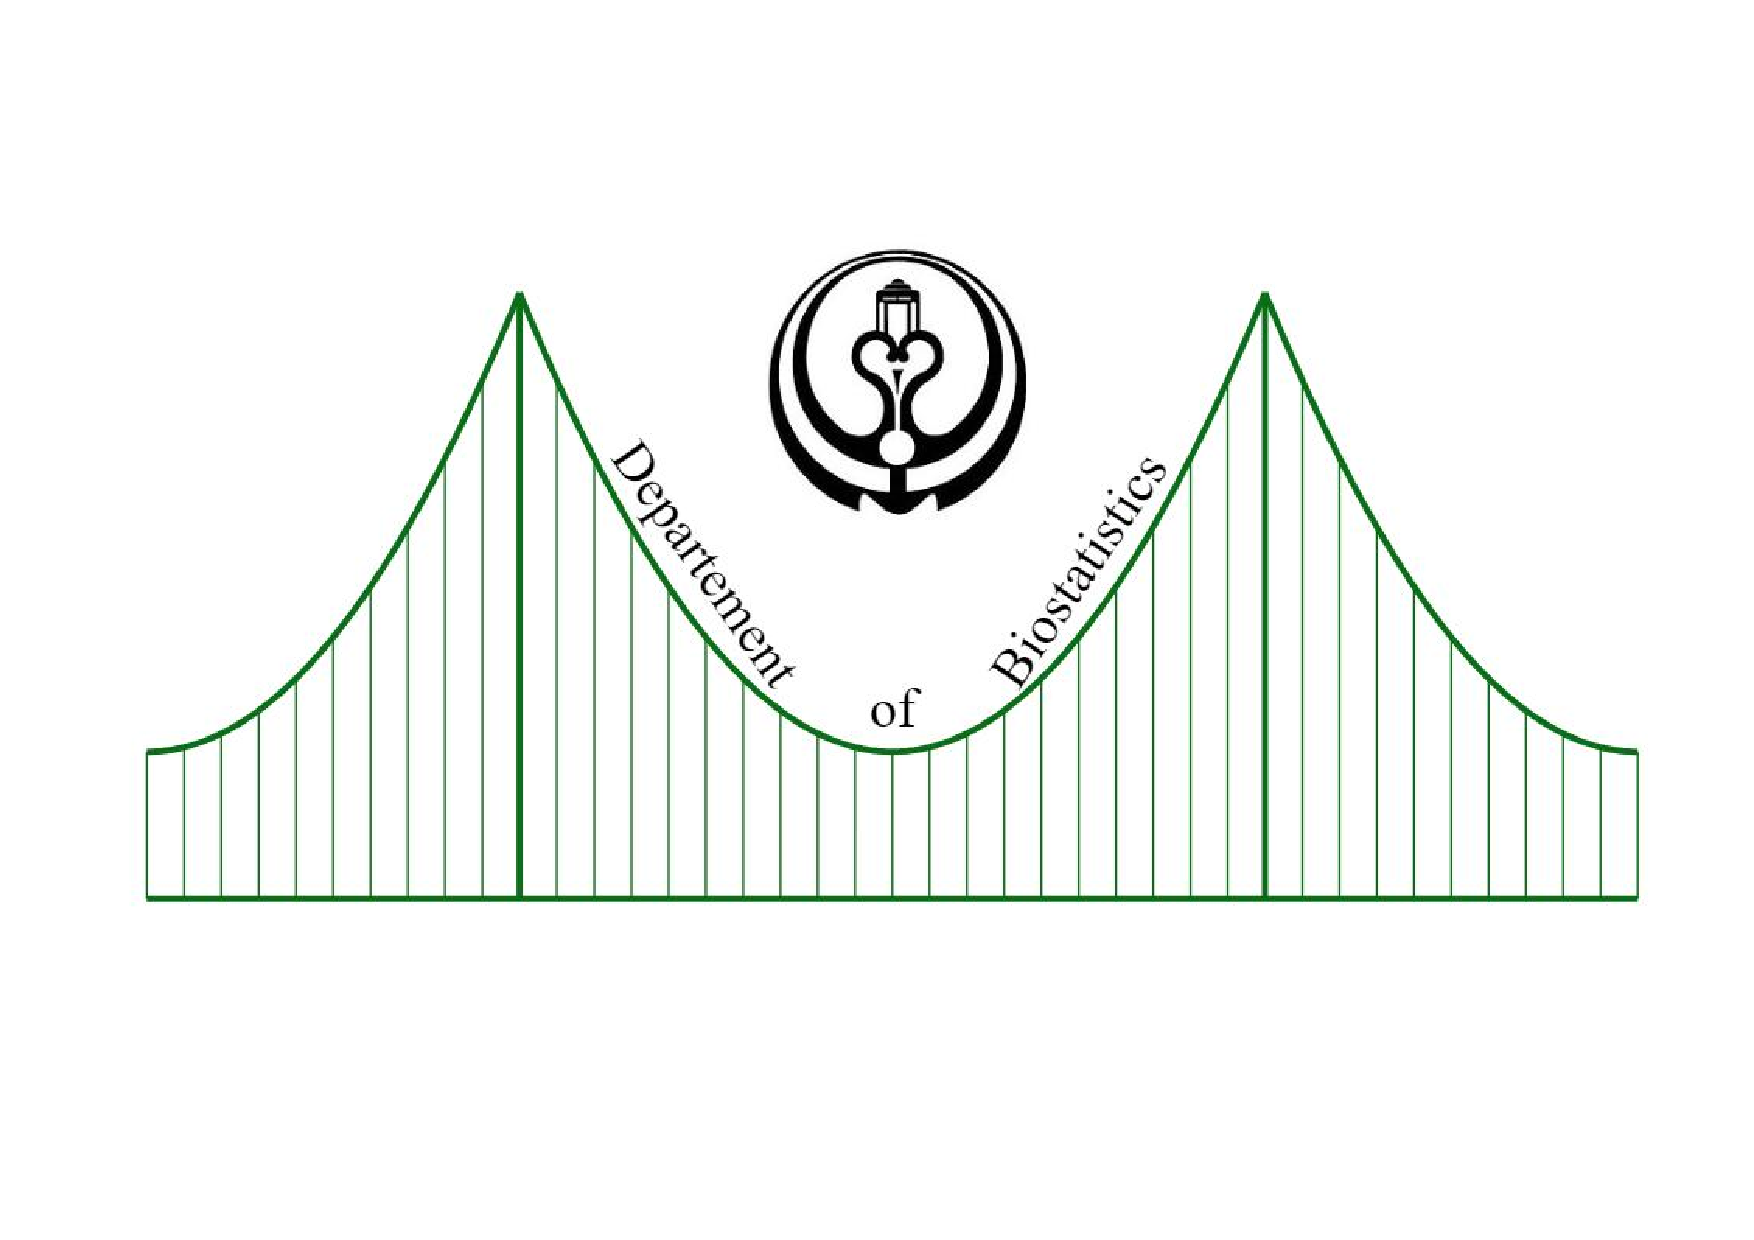
\includegraphics[height = 5cm, width = 8cm]{Logo_Sums_BioStatistics.pdf}\\  R Programming WorkShop}

\author{habib ezzat abadi}
\institute{Shiraz University of Medical Scinece}
\hypersetup{
pdfauthor = {H_Ezzatabadi},
pdftitle = {R WorkShop},
pdfsubject = {1402-1403},
pdfkeywords = {R, Programming},
pdfpagemode = {FullScreen}
}
\defbeamertemplate*{footline}{shadow theme}{%
\leavevmode%
\hbox{\begin{beamercolorbox}[wd=.5\paperwidth,ht=2.5ex,dp=1.125ex,leftskip=.3cm plus1fil,rightskip=.3cm]{author in head/foot}%
    \usebeamerfont{author in head/foot}\hfill\insertshortauthor
\end{beamercolorbox}%

\begin{beamercolorbox}[wd=.5\paperwidth,ht=2.5ex,dp=1.125ex,leftskip=.3cm,rightskip=.3cm plus1fil]{title in head/foot}%
    \usebeamerfont{title in head/foot}\insertshorttitle\hfill%
\insertframenumber\,/\,\inserttotalframenumber
\end{beamercolorbox}}%
\vskip0pt%
}
\IfFileExists{upquote.sty}{\usepackage{upquote}}{}
\begin{document}


\frame[plain]{\maketitle}
%%%%%%%%%%%%%%%%%%%%%%%%%%%%%%%%%

\begin{frame}{Outline}
    \tableofcontents
\end{frame}

%%%%%%%%%%%%%%%%%%%%%%%%%%%

\begin{frame}{A Brief History of R}
 \begin{itemize}
\item 1976 S-Bell Labs: Fortran 
\begin{itemize}
\item[-]John Chambers
\item[-] Rick Becker
\item[-] Allan Wilks 
\end{itemize}
\item 1988 S Version 3: C language 
\begin{itemize}
    \item[-] John Chambers 
\end{itemize}
\item 1991 R Created 
\begin{itemize}
    \item[-] Ross Ihaka
    \item[-] Robert Gentelman 
\end{itemize}
\item 1993 R Announced
\item 2000 R Version 1 Released
\item 2020 8th rank of programming languages
\item 2023 16th rank of Programming languages
 \end{itemize}   
\end{frame}

\begin{frame}
    \tikzstyle{terminal} = [rectangle, minimum width = 2cm, minimum height = 2cm, 
    rounded corners, text centered, draw = black, fill = yellow!20, inner sep = 0pt]
    \tikzstyle{arrow} = [thick, ->, >=stealth]

\begin{tikzpicture}[node distance = 2cm]
% First Rows
\node (sas1) [terminal] {
\includegraphics[width=0.2\textwidth]{hadley_wickham.pdf}};    
\node (minitab1) [terminal, right of = sas1, xshift = 6cm] {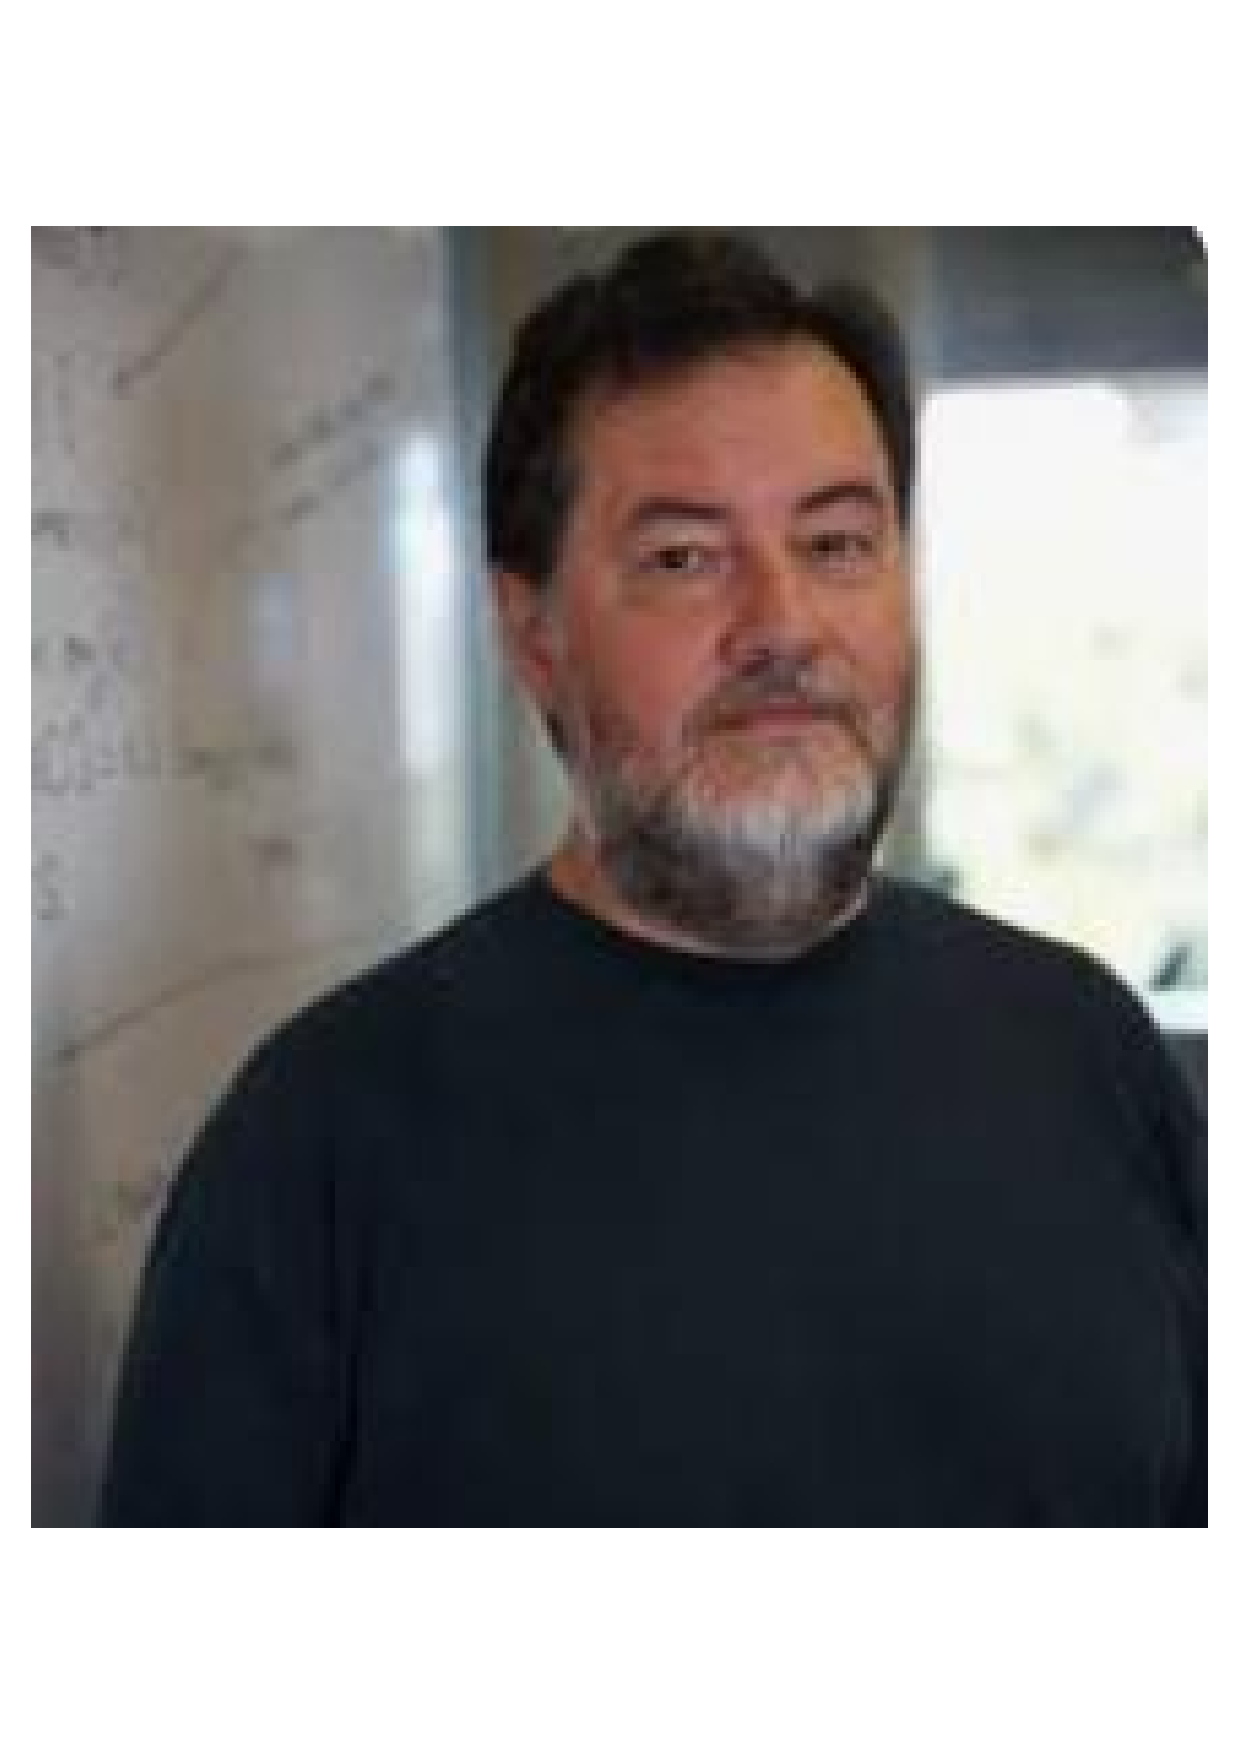
\includegraphics[width=.2\textwidth]{ross_ihaka.pdf}}; 
% second Rows
\node (rr) [terminal, below of = sas1, xshift = 4cm, yshift = -0.75cm] {
\includegraphics[width = 0.3\textwidth]{RLogo.pdf}};
\node (r1) [terminal, below of = rr, xshift = -3.5cm, yshift = -0.75cm] {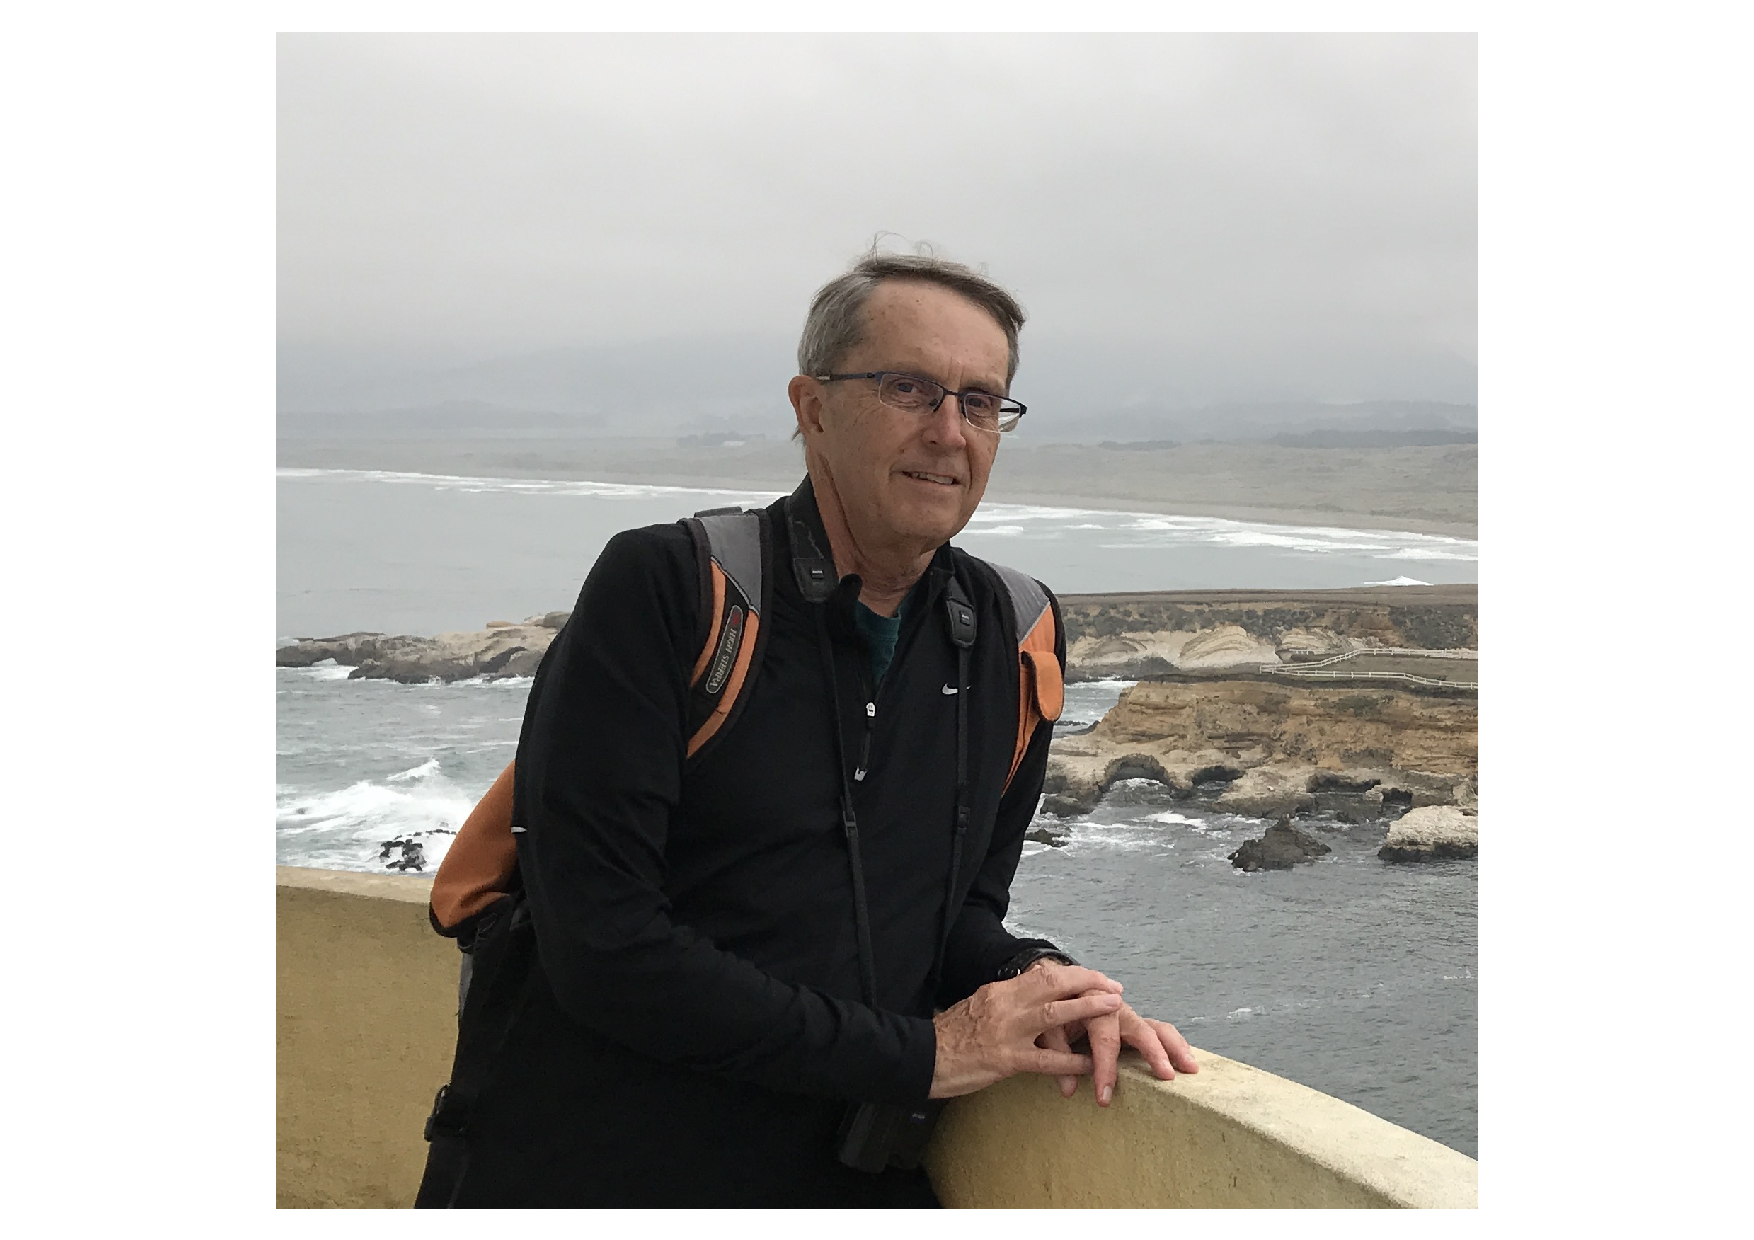
\includegraphics[width=0.2\textwidth]{john_chambers.pdf}};  
% third rows
\node (matlab1) [terminal, below of = minitab1, yshift = -3.5cm] {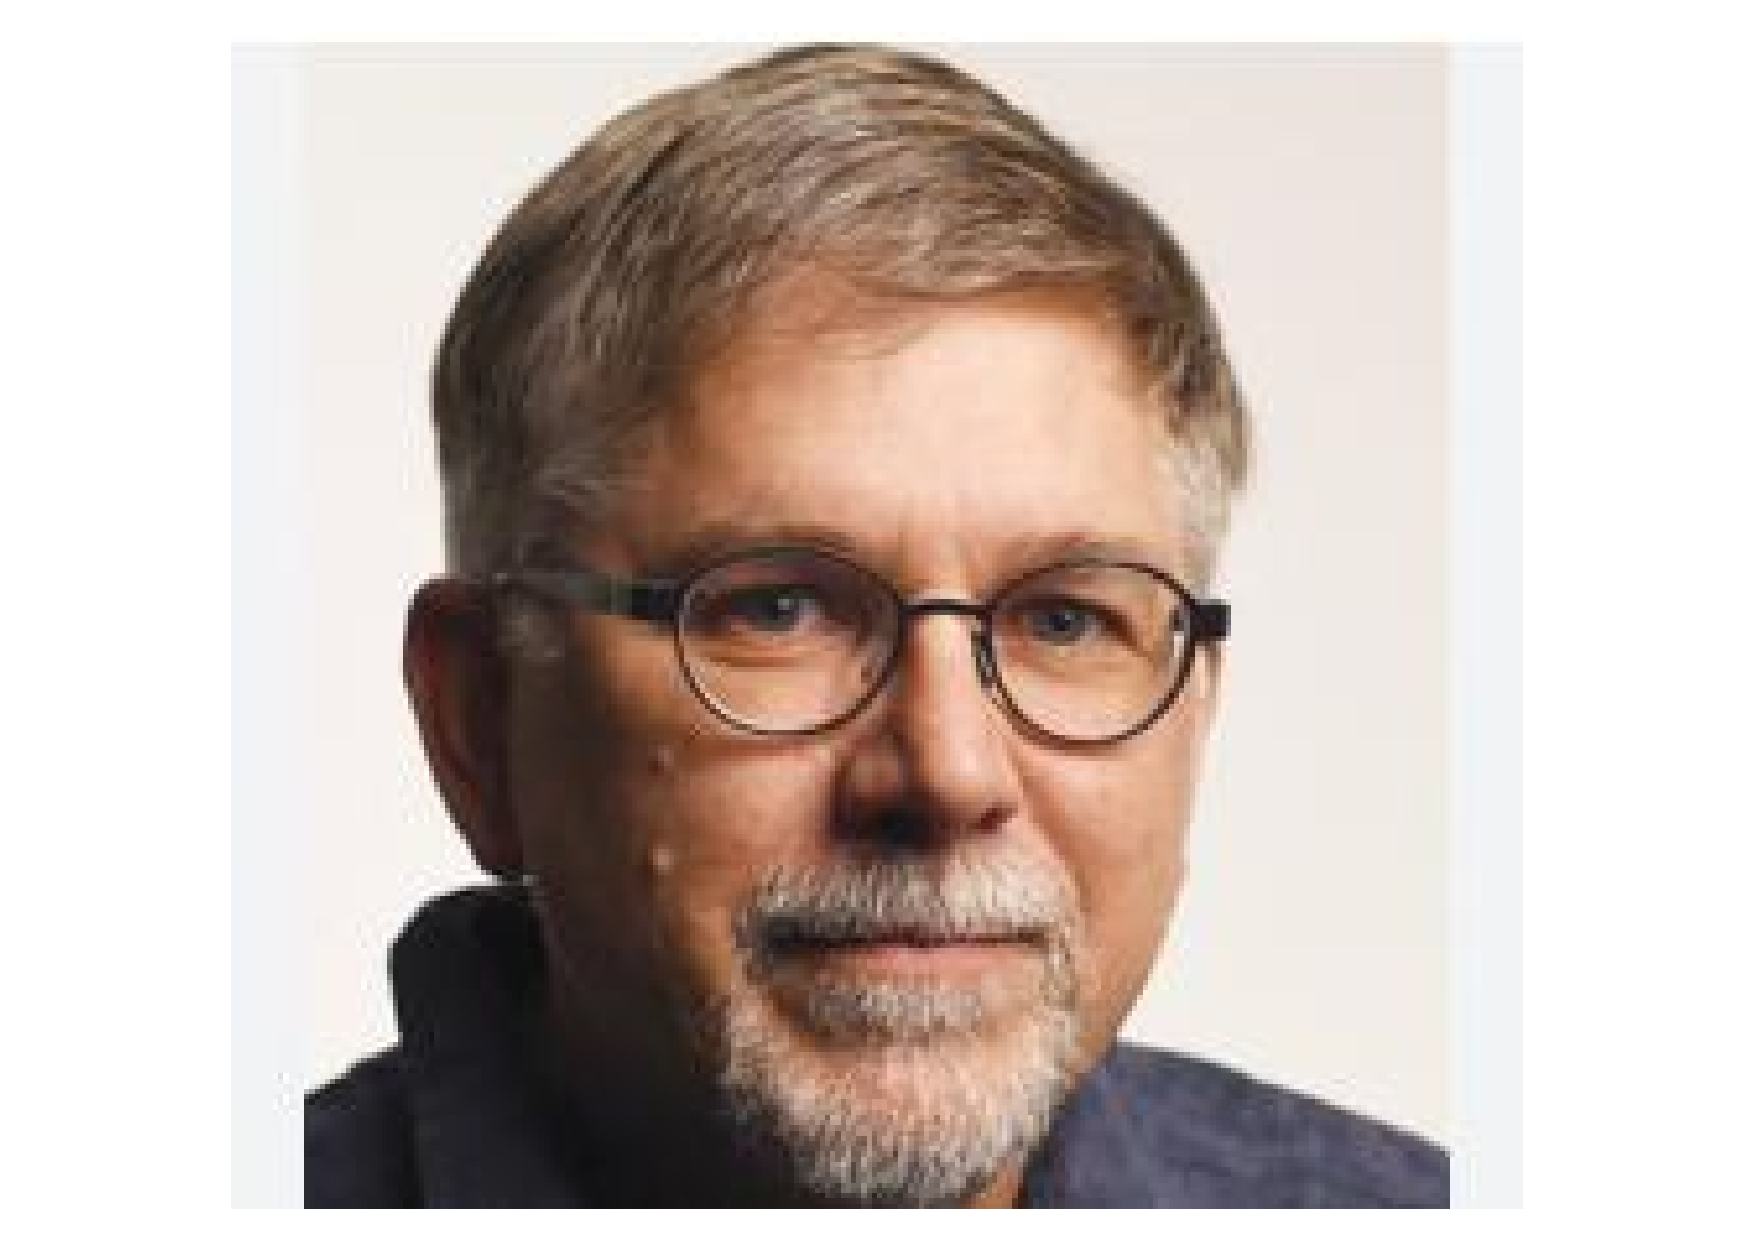
\includegraphics[width=0.2\textwidth]{RobertGentelman.pdf}};  
\draw [arrow] (sas1) -- (rr);
\draw [arrow] (minitab1) -- (rr); 
\draw [arrow] (matlab1) -- (rr);
\draw [arrow] (r1) -- (rr); 
\end{tikzpicture}
\end{frame}
\begin{frame}{Why R?}

    \tikzstyle{terminal} = [rectangle, minimum width = 2cm, minimum height = 2cm, 
    rounded corners, text centered, draw = black, fill = yellow!20]
    \tikzstyle{other} = [ellipse, minimum width = 2cm, minimum height = 1cm, 
    rounded corners, text centered, draw = black, fill = blue!20]
    \tikzstyle{arrow} = [thick, ->, >=stealth]

\begin{tikzpicture}[node distance = 2cm]
% First Rows
\node (sas1) [other] {SAS};  \node (spss1) [other, right of = sas1, xshift = 1cm]{SPSS};  \node (minitab1) [other, right of = spss1, xshift = 1.5cm] {MINITAB}; 
% second Rows
\node (gr1) [other, below of = sas1, xshift = -1cm, yshift = -0.75cm] {GraphPad Prism};  \node (r1) [terminal, below of = spss1, yshift = -0.75cm] {R};  \node (stat1) [other, below of = minitab1, yshift = -0.75cm] {STATA}; 
% third rows
\node (matlab1) [other, below of = gr1, yshift = -0.75cm] {MATLAB};   \node (st1) [other, below of = r1, yshift = -0.75cm] {STATISTICA};  \node (ncss1) [other, below of = stat1, yshift = -0.75cm] {NCSS};
\end{tikzpicture}



\end{frame}
\section{Conditional structures}
\begin{frame}{Types of conditional structures in R}
    \begin{alertblock}{type of conditional structures in R}
        \begin{itemize}
            \item if
            \item if-else 
            \item ifelse
        \end{itemize}
    \end{alertblock}
\end{frame}




\subsection{if}





\begin{frame}{if structure}
\begin{block}{Why We Using if structure?}
    Sometimes we need a certain task to be done only when a condition is met, otherwise we want the normal flow of the program to be maintained if the condition is not met.
\end{block}
\end{frame}

%%%%%%%%%%%%%%%%%%%%%%%%%%%%%%%%%%%
\begin{frame}{Example of if structure}
\begin{exampleblock}{Ex. (i)}
Get a number from the user. If the remainder of this number is divided by 5 ‌is 2 or 3, print "Great" in the output, otherwise, do nothing.
\end{exampleblock}
\end{frame}



\begin{frame}{Labs}
    \alert{{\Large Go to the coding environment $\rightarrow$}}
\end{frame}













\subsection{if-else}
\begin{frame}{if-else}
    \begin{block}{if-else}
        But there are times when we need to change the path of the program for any answer when we check the condition. And it is even possible to obtain different modes for different modes.
    \end{block}
\end{frame}

%%%%%%%%%%%%%%%%%%%%%%%%%%%%%%%%%%%%%%
\begin{frame}{structure of if-else}
    \begin{block}{CodeBlock}
\begin{align*}
    & \text{if (condition) \{} \\
    & \text{command1} \\
    & \text{command2} \\
    & \dots \\
    & \text{\}}\text{~else\{}\\
    & \text{if \{}\\
    & \dots \\
    & \text{\}}
\end{align*}
\end{block}
    
\end{frame}
%%%%%%%%%%%%%%%%%%%%%%%%%%%%%%%%%%%%%%%%%%%%%%%

\begin{frame}{Example}
\begin{exampleblock}{Ex. (ii)}
take a number from the user, with the condition that it is greater than 20, then if the remainder of this number is zero compared to five numbers, print the value of "A" in the output, if
    was 1, print the value of "B" in the output, if it was 2, print the value of "CC" in the output and if it was 3, print the value of "C" in the output, and finally, if it was 4
    Print the value of "D" in the output.
\end{exampleblock}
\end{frame}


\begin{frame}{Labs}
    \alert{{\Large Go to the coding environment $\rightarrow$}}
\end{frame}

%%%%%%%%%%%%%%%%%%%%%%%%%%%%%%%%%%%%%%%%%%%%





\subsection{ifelse}

\begin{frame}{ifelse}

    \begin{block}{ifelse}
        
    
Sometimes we are faced with a binary situation, if the condition is met, one thing will happen, and if the condition
    If it is not established, one more thing will happen and our conditional structure will not extend further.
    R programming language has defined a very simple structure for this mode
    by the name of ifelse. 
\end{block}
\end{frame}



\begin{frame}{Example}
\begin{exampleblock}{Ex. (iii)}
Get an input from the user. If the input was even, it returns the value "even" and otherwise it returns the value "odd".
\end{exampleblock}
\end{frame}







\begin{frame}{Labs}
    \alert{{\Large Go to the coding environment $\rightarrow$}}
    \end{frame}


%%%%%%%%%%%%%%%%%%%%%%%%%%%%%%%%%%%%%%%%%%%
\section{Loops in R Programming}
\begin{frame}{Why Using Loops in Programming?}

\begin{alertblock}
{\large loops are an essential tool in programming that allow you to execute a block of code repeatedly until a certain condition is met. They are useful for performing repetitive 
tasks without writing the same code multiple times.}
\end{alertblock}
\end{frame}


%%%%%%%%%%%%%%%%%%%%%%%%%%%%%%%%%%%%%%%


\begin{frame}{Loops in R}
\begin{itemize}
    \item Using while loop
    \item Using repeat loop
    \item Using for loop
\end{itemize}
\end{frame}
\subsection{while loop}
\begin{frame}{why do we use while loop?}
    \begin{figure}[H]
        \centering
    \tikzstyle{decision} = [rectangle, draw, text centered, rounded corners, minimum height=2em]
    \tikzstyle{data} = [rectangle, draw, text centered, minimum height=2em]
    \tikzstyle{terminator} = [ellipse, draw, text centered, minimum width = 2em, minimum height=1em]
    \begin{tikzpicture}[->,>=stealth', auto, thick]
        \node [terminator, fill=yellow!20] at (0,0) (start) {\textbf{Logical condition}};
        \node [data, fill=green!20, yshift = -2cm] at (0,-2) (data) {Code Block};
        \node [decision, fill=red!20] at (0,-5) (decision) {End};
        \draw [->, green] (start.south) -- (data.north);
        \draw [->, blue] (start.east) to [out = 50, in = 30] (decision.east);
        \draw [->, red] (data.west) to [out = 130, in = 150]  (start.west);
        \node[draw=none] at (-0.5, -2.5) (no) {True};  
        \node [draw = none] at (1.75, -1.5) (yes) {False};  
    \end{tikzpicture}
\end{figure}
\end{frame}
\begin{frame}
    
    \begin{exampleblock}{Ex (iv).}
        \label{ex1}
\begin{align*}
    & f(x) = \exp(x) - x^2, \\
    & \text{if} \quad f(x) = 0 \implies x = ~?
\end{align*}
        
    \end{exampleblock}
\end{frame}

\begin{frame}{Labs}
\alert{{\Large Go to the coding environment $\rightarrow$}}
\end{frame}
\subsection{repeat loop}

\begin{frame}{why do we use repeat loop?}
    \begin{figure}
        \centering
    \tikzstyle{decision} = [rectangle, draw, text centered, rounded corners, minimum height=2em]
    \tikzstyle{data} = [rectangle, draw, text centered, minimum height=2em]
    \tikzstyle{terminator} = [diamond, draw, text centered, minimum height=2em]
    \begin{tikzpicture}[->,>=stealth', auto, thick]
        \node [data, fill=yellow!20] at (0,0) (data) {\textbf{Code Block}};
        \node [terminator, fill=green!20, yshift = -1cm] at (0,-2) (start) {\textbf{Logical condition}};
        \node [decision, fill=red!20, yshift = -1cm] at (0,-5) (decision) {End};
        \draw [->, green] (data.south) -- (start.north);
        \draw [->, blue] (start.east) to [out = 50, in = 30] (decision.east);
        \draw [->, red] (start.west) to [out = 130, in = 150]  (data.west);
        \node[draw=none] at (2.3, -4.5) (no) {True};  
        \node [draw = none] at (-1.75, -1.5) (yes) {False};  
    \end{tikzpicture}
\end{figure}
\end{frame}
\begin{frame}
    \begin{exampleblock}{Ex (v).}
By referring to the example in slide (\ref{ex1}), get the numerical answer using loop repeat.
    \end{exampleblock}
\end{frame}


\begin{frame}{Labs}
    \alert{{\Large Go to the coding environment $\rightarrow$}}
    \end{frame}

\subsection{For loop}

\begin{frame}{Why do we use For loop?}
    \begin{figure}
        \centering
    \tikzstyle{decision} = [rectangle, draw, text centered, rounded corners, minimum height=2em]
    \tikzstyle{data} = [rectangle, draw, text centered, minimum height=2em]
    \begin{tikzpicture}[->,>=stealth', auto, thick]
        \node [data, fill=yellow!20] at (0,0) (p1) {\textbf{Initialization}};
        \node [decision, fill=green!20] at (-1,-2) (p2) {\textbf{Code Block}};
        \node[decision, fill = blue!20] at (0, -4) (p3) {\textbf{Last iteration?}};
        \node [decision, fill=red!20] at (-2,-6) (p4) {End};
        \draw [->, green] (p1) -- (p2);
        \draw [->, blue] (p2) -- (p3);
        \draw [->, red] (p3) -- (p4);
        \draw [->, black] (p3.east) to [out = 50, in = 30] (p1.east);
        \node[draw=none] at (2.7, -1.5) (no) {No};  
        \node [draw = none] at (-1.5, -5) (yes) {Yes};  
    \end{tikzpicture}
\end{figure}
\end{frame}

\begin{frame}
    \begin{exampleblock}{Example (vi):}
Generate a matrix with 10 rows and 10 columns of integer values.
\begin{itemize}
    \item[a)] Calculate the row sum of this matrix using the for loop.
    \item[b)] Using the \it{"next"} command, if the sum of a row is more than 500, do not print that row sum in the output. 
    \item[c)] If a row is calculated whose sum is greater than 600, the loop will stop. using the command (break) 
\end{itemize}
    \end{exampleblock}
\end{frame}
\begin{frame}{Labs}
    \alert{{\Large Go to the coding environment $\rightarrow$}}
    \end{frame}

    
    %%%%%%%%%%%%%%%%%%%%%%%%%%%%%%%%%%%%%%%%%%%%%%%%%%%%%%%%%%%%%


    \section{Fanctional Programming}
    

    \begin{frame}{Why do we need functions in Programming?}
    \textcolor{blue}{Functions in programming are essential for several reasons:}

    \begin{block}{Functional Programming}
        \begin{enumerate}

            \item \textcolor{red}{Code Reusability:}~ Functions allow us to write a piece of code once and reuse it multiple times. This can save a lot of time and effort, especially in large programs.
            
            \item \textcolor{red}{Modularity:}~ Functions help to break down large programs into small, manageable parts. This makes the code easier to understand, debug, and maintain.
            
            \item \textcolor{red}{Abstraction:}~ Functions hide the details of their operation, allowing us to use them without knowing exactly how they work. This is a key principle of software design known as abstraction.
            
        \end{enumerate}
    \end{block}
\end{frame}
%%%%%%%%%%%%%%%%%%%%%%%%%%%%%%%%%%%


\begin{frame}{Functional Programming}
\begin{block}{continue about Functional Programming}
    \begin{enumerate}
        \setcounter{enumi}{3}
        \item  \textcolor{red}{Namespace Separation:}~ Variables defined inside a function are not visible outside the function. This helps to prevent naming conflicts in our code.
            
        \item \textcolor{red}{Testing and Debugging:}~ It's easier to test and debug small functions than large monolithic code blocks. If a problem occurs, it's easier to pinpoint the issue in a small, isolated function.
        
        \item \textcolor{red}{Code Readability:}~ Well-named functions can make the code more readable and self-explanatory, improving its understandability.
        
    \end{enumerate}
\end{block}

\end{frame}
    %%%%%%%%%%%%%%%%%%%%%%%%%%%%

    \begin{frame}{Functional Programming}
    \begin{alertblock}{summary}
        In summary, functions are a fundamental building block of programming that help us write better, more manageable, and efficient code. They are a key part of structured and object-oriented programming.
    \end{alertblock}
    \end{frame}

%%%%%%%%%%%%%%%%%%%%%%%%%%%%%%%%%%%%%%%%%%%%%%%%%%%%%%%%%%%%


\subsection{A short look at algorithm writing}
\begin{frame}{Creator}
    \small{Abullah Mohammad bin Musa al Khwarizmi, Who is often referred to as "The Father of Algebra"}
    \begin{figure}[H]
        \centering
        
    
\includegraphics[width = 6cm]{kharazmi.pdf}
    
    \end{figure}

    %%%%%%%%%%%%%%%%%%%%%%%%%%%%%%%%%%%%%%

\end{frame}
\begin{frame}{Definition}

    \begin{definition}
        An algorithm is a process or set of rules to be followed in calculations or other problem-solving operations, especially by a computer. It's a sequence of instructions that a computer must perform to solve a well-defined problem. It essentially defines what the computer needs to do and how to do it. Algorithms can instruct a computer how to perform a calculation, process data, or make a decision.
    \end{definition}

\end{frame}


%%%%%%%%%%%%%%%%%%%%%%%%%%%%%%%%%%%%%%%%%%%%%%%%%%%%%%%%%%%%%%

\begin{frame}{Why do we need algorithms?}
    \textcolor{blue}{ Algorithms are crucial in functional programming for several reasons:}
    \begin{block}
       
\begin{enumerate}
    

\item \textcolor{red}{Predictability:}~ Algorithms provide a clear sequence of steps to solve a problem, which makes the program's behavior predictable.

\item \textcolor{red}{Efficiency:}~ Efficient algorithms can significantly reduce the time and space complexity of your program, making it run faster and consume less memory.

\item \textcolor{red}{Problem Solving:}~ Algorithms are essential tools for solving complex problems in programming. They provide a structured approach to problem solving, which is particularly important in functional programming where side effects are avoided.

\end{enumerate}

\end{block}
\end{frame}

%%%%%%%%%%%%%%%%%%%%%%%%%%%%%

\begin{frame}{Algorithms}
\begin{block}{continue about Algorithms}
    \begin{enumerate}
        \setcounter{enumi}{2}

\item \textcolor{red}{Code Reusability:}~ Similar to functions, algorithms can be reused across different parts of a program or even different programs. This can save a lot of time and effort in development.

\item \textcolor{red}{Understanding and Communication:}~ Algorithms provide a way for programmers to communicate their ideas effectively. They are language-agnostic, meaning they can be implemented in any programming language.

    \end{enumerate}
\end{block}
\end{frame}

%%%%%%%%%%%%%%%%%%%%%%%%%%%%%%%%%%%%%%%%%
\begin{frame}{Algorithms}
\begin{alertblock}{Summary}
    In summary, algorithms are a fundamental part of functional programming and programming in general. They help us solve problems efficiently and effectively, and are a key tool in a programmer's toolkit.

\end{alertblock}
\end{frame}
%%%%%%%%%%%%%%%%%%%%%%%%%%%%%%%%%%%%%%%%%%%%%%%%%%%%

\begin{frame}{Algorithms}
\begin{exampleblock}{Ex. (vii)}
    Write an algorithm that takes a number from the user and determines if this number is prime or not?
\end{exampleblock}
\end{frame}

%%%%%%%%%%%%%%%%%%%%%%%%%

\begin{frame}{Algorithms}
    \begin{algorithm}[H]
        \SetAlgoLined
        \KwResult{True or False}
         \textbf{Function} isPrime(n):\\
         \eIf{n is less than 2}{
          \Return False\;
          }{
           \For{i from 2 to n}{
            \If{n mod i equals 0}{
             \Return False\;
             }
           }
           \Return True\;
          }
         \caption{Prime Check}
        \end{algorithm}
\end{frame}

%%%%%%%%%%%%%%%%%%%%%%%%%%%%%%%%%%%%%%%%%

\subsection{function}
\begin{frame}
\begin{alertblock}{Objects and functions in R Programming}
    \begin{itemize}
        \item Everything that exists is an object.
        \item Everything that happens is a function call.
    \end{itemize}
    \begin{quote}
        John Chambers
    \end{quote}
\end{alertblock}
\end{frame}



%%%%%%%%%%%%%%%%%%%%%%%%%%%%%%%%%%%%%%%%%%%%%%%%%%%%

\begin{frame}{function}
    \begin{block}{Elements of a function}
        \begin{itemize}
            \item formals
            \item body
            \item environment
        \end{itemize}
        
    \end{block}
\end{frame}
%%%%%%%%%%%%%%%%%%%%%%%%%%%%%%%%%%%%%%%%%%%%%%%%%%


\begin{frame}{formals of function}
    \begin{block}{formals}
        These are the arguments of the function. They control how you can call the function. When a function is invoked, you can pass values to it through these arguments.
    \end{block}
    \begin{exampleblock}{EX. (viii)}
        \label{ex8}
        \begin{align*}
            & \text{myfun <- function(x1, x2, x3) \{}\\
            & \text{temp1 = x1 * x2} \\
            & \text{return(temp1)}\\
            & \}
        \end{align*}
    \end{exampleblock}
\end{frame}
%%%%%%%%%%%%%%%%%%%%%%%%%%%%%%%%%%%

\begin{frame}{Body of functions}
    \begin{block}{Body}
        This is the code inside the function. It contains the sequence of statements that the function will execute when it is called.
    \end{block}
\end{frame}

%%%%%%%%%%%%%%%%%%%%%%%%%%%%%%%%%%%%
\begin{frame}{Environment of functions}
    \begin{block}{Environment}
        This is the "map" of the location of the function's variables. When a function is executed, it creates a new environment to hold its local variables.
    \end{block}

    
\end{frame}

%%%%%%%%%%%%%%%%%%%%%%%%%%%%
\begin{frame}{lazy evaluation}
    \begin{block}{lazy evaluation}
        Lazy evaluation, also known as call by need, is a technique used in R programming where the evaluation of an expression is delayed until its value is absolutely needed. This means that in R, an expression is not evaluated when it is not used. 
        For instance, if a function argument is not used in the function, R will not evaluate it. This strategy increases the efficiency of the program, especially when used iteratively, as it avoids repeated evaluations. 
    \end{block}
\end{frame}


%%%%%%%%%%%%%%%%%%%%%%%%%%%%%%%%%%%%%%%%%%%%%%%%%

\begin{frame}{Primitive functions}

\begin{block}{Primitive functions}
    In R programming, primitive functions are a special type of function that are implemented at a low level for performance reasons. They are only found in the base package and include language elements like "if" and "for", operators like "and" and "\$", and mathematical functions like "exp" and "sin".
\end{block}
\end{frame}
%%%%%%%%%%%%%%%%%%%%%%%%%%%%%%%%%%%%%%%%%

\begin{frame}{Primitive functions}
\textcolor{blue}{Primitive functions have several unique characteristics:}

    \begin{alertblock}{Primitive funcitons}
\begin{itemize}
    \item They operate at a low level, which can make them more efficient.
    \item They have different rules for argument matching.
    \item They do not allow any R-code in the function.
    \item They use a special technique for accessing C-code.
\end{itemize}
\end{alertblock}
\end{frame}
%%%%%%%%%%%%%%%%%%%%%%%%%%%%%%%%%%%%%%%%%%%%%

\begin{frame}{Generic functions}
\begin{block}{Generic functions}

    In R programming, generic functions play a crucial role in object-oriented programming. They are functions that behave differently based on the class of the input. This is known as polymorphism.

Generic functions use a system called "S3", which was introduced in "S" version 3. You can identify an S3 generic function because its entire body is a call to the R function "UseMethod". For example, "plot" and "summary" are generic functions.
\end{block}
\end{frame}


%%%%%%%%%%%%%%%%%%%%%%%%%%%%%%%%%%%%


\section{Parallel Programming in R}
\begin{frame}{Introduction}
\begin{block}{basic concepts}
Let’s be a little more formal.
Consider that we have a series of functions to run, f1, f2, etc.
Serial processing means that f1 runs first, and until f1 completes, nothing else can run. Once f1 completes, f2 begins, and the process repeats.
Parallel processing (in the extreme) means that all the f$\#$ processes start simultaneously and run to completion on their own.
    \end{block}
\end{frame}

%%%%%%%%%%%%%%%%%%%%%%%%%%%%%%%%%%%%%%%

\begin{frame}{Prallel Programming}
\begin{block}{The Serial-parallel scale}
A problem can range from “inherently serial” to “perfectly parallel".
An “inherently serial” problem is one which cannot be parallelized at all, 
for example, if f2 depended on the output of f1 before it could begin, 
even if we used multiple computers, we would gain no speed-ups.
On the other hand a “perfectly parallel” problem is one in which 
there is absolutely no dependency between iterations; most of the 
apply calls or simulations we’ve discussed in this WorkShop fall into this category. In this case, 
any f can start at any point and run to completion regardless of the status of any other f.
\end{block}
\end{frame}

%%%%%%%%%%%%%%%%%%%%%%%%%%%%%%%%%%%%%%%%%%

\begin{frame}{Parallel Programming}
\begin{block}{Terminology}
\begin{itemize}
    \item A core is a general term for either a single processor on your own computer (technically you only have one processor, but a modern processor like the i7 can have multiple cores - hence the term) or a single machine in a cluster network.
    \item  A cluster is a collection of objecting capable of hosting cores, either a network or just the collection of cores on your personal computer.
    \item A process is a single running version of R (or more generally any program). Each core runs a single process.
\end{itemize}  
\end{block}  
\end{frame}

%%%%%%%%%%%%%%%%%%%%%%%%%%%%%%

\begin{frame}{The parallel package}
    \begin{block}{The parallel package}

      There are a number of packages which can be used for parallel processing in R. Two of the earliest and strongest were multicore and snow. However, both were adopted in the base R installation and merged into the parallel package.  
    \end{block}
    
\end{frame}
%%%%%%%%%%%%%%%%%%%%%%%%%%%%%%%%%%%%

\begin{frame}{Initial Coammands}
\begin{block}{Initial Coammands}
    \begin{align*}
        & \text{library(parallel)} \\
        & \text{detectCores()}
    \end{align*}   
\end{block}
\end{frame}

%%%%%%%%%%%%%%%%%%%%%%%%%%%%%%%%%%%%%%%%

\subsection{Types of Parallel Programming}
\begin{frame}{Types of Parallel Programming}
    \begin{itemize}
        \item SOCKET approach
        \item FORK approach
    \end{itemize}
\end{frame}
%%%%%%%%%%%%%%%%%%%%%%%%%%%%%%%%%%%%%%%%%%%%%%%%

\begin{frame}{Types of Parallel Programming}
\begin{block}{Types of Prallel Programming}
\begin{itemize}
    \item The socket approach launches a new version of R on each core. Technically this connection is done via networking (e.g. the same as if you connected to a remote server), 
    but the connection is happening all on your own computer mention this because you may get a warning from your computer asking whether to allow R to accept incoming connections, you should allow it.
    \item The forking approach copies the entire current version of R and moves it to a new core.
\end{itemize}
\end{block}
\end{frame}

%%%%%%%%%%%%%%%%%%%%%%%%%%%%%%%%%%%%%%%%%%%%
\begin{frame}{SOCKET}
    There are various pro’s and con’s to the two approaches:

\begin{alertblock}{PROS and CONS for Socket approach}
    \begin{itemize}
        \item \textcolor{blue}{Works on any system (including Windows).}
        \item \textcolor{blue}{Each process on each node is unique so it can’t cross-contaminate.}
        \item \textcolor{red}{Each process is unique so it will be slower}
        \item \textcolor{red}{Things such as package loading need to be done in each process separately. Variables defined on your main version of R don’t exist on each core unless explicitly placed there.}
        \item \textcolor{red}{More complicated to implement.}
    \end{itemize}

\end{alertblock}
\end{frame}
%%%%%%%%%%%%%%%%%%%%%%%%%%%%%%%%%%%%%%%%%%%%%




\begin{frame}{Forking}
    
\begin{alertblock}{PROS and CONS for Forking approach}
    \begin{itemize}
        \item \textcolor{red}{Only works on POSIX systems (Mac, Linux, Unix, BSD) and not Windows.}
        \item \textcolor{red}{Because processes are duplicates, it can cause issues specifically with random number generation (which should usually be handled by parallel in the background) or when running in a GUI (such as RStudio). This doesn’t come up often, but if you get odd behavior, this may be the case.}
        \item \textcolor{blue}{Faster than sockets.}
        \item \textcolor{blue}{Because it copies the existing version of R, your entire workspace exists in each process.}
        \item \textcolor{blue}{Trivially easy to implement.}
    \end{itemize}

\end{alertblock}
\end{frame}
%%%%%%%%%%%%%%%%%%%%%%%%%%%%%%%%%%%%%%%%%%%%%%%%%%%


\begin{frame}{Labs}
    \begin{alertblock}{Labs Links}
        In order to be able to access the codes and examples, you can visit these two links;\\
        \href{https://github.com/stats9/R_Fancy/blob/master/WorkShopSums/Beemer_Present/WorkShopSums_code_template.ipynb}{First link}\\
        \href{https://github.com/stats9/R_Fancy/blob/master/WorkShopSums/WorkShop_1_Sums_R_Programming.md}{second link.}
    \end{alertblock}

\end{frame}

\end{document}

